\section{Resoconto attività di verifica}
In questa sezione vengono descritti e analizzati gli esiti delle attività
di verifica svolte su tutti i documenti che vengono consegnati nelle varie 
revisioni di avanzamento del progetto.
\subsection{Revisioni}
\subsubsection{Revisione dei requisiti}
\paragraph{Tracciamento dei casi d'uso e dei requisiti}\mbox{}\\
Per facilitare il tracciamento delle relazioni fra casi d'uso e requisiti che
fra requisiti e fonti, il gruppo ha deciso di utilizzare il software PragmaDB.

\paragraph{Analisi statica dei documenti}\mbox{}\\
L'analisi dei documenti mediante \textit{Walkthrough}\glo{} ha portato 
all'individuazione di alcuni errori frequenti a partire dai quali è stata 
stilata una lista di controllo interna. In questo modo sarà possibile applicare
l'\textit{Inspection}\glo{} per le future attività di verifica.

\subsubsection{Revisione di progettazione}
\paragraph{Analisi statica del codice}\mbox{}\\
La stesura del codice è supportata dai plugin dell'editor Visual Studio Code. I plugin rilevanti in ambito di verifica sono due:
\begin{itemize}
	\item \textbf{ESLint v1.8.1}: linter per il linguaggio JavaScript;
	\item \textbf{Solidity v0.0.49}: linter per il linguaggio Solidity.
\end{itemize}
 I linter hanno aiutato notevolmente la stesura di codice sintatticamente corretto e alla standardizzazione del codice scritto, che risulta più uniforme; inoltre hanno facilitato parzialmente il processo di debugging.
 
\subsubsection{Revisione di qualifica}
\paragraph{Test}\mbox{}\\
Abbiamo preparato i test di accettazione e di sistema, i quali sono riportati nella sezione: "Test: stato e specifica". Tali test verranno implementati per la revisione di accettazione.\\
%aggiungere label a sezione Specifica dei test
I test di integrazione e di unità sono in fase di costruzione.\\
Abbiamo creato e implementato test di unità sui contratti di backend per controllare la correttezza del codice e guidarne l'implementazione. 
Per la preparazione dei test sono serviti i seguenti strumenti:
\begin{itemize}
	\item \textbf{Truffle v5.0.4}: è usato il comando \texttt{truffle test};
\end{itemize}
\subsection{Revisione di accettazione}
\paragraph{Test}\mbox{}\\
I test di integrazione e di unità sono stati completati e ne è stato verificato l'esito.
Test di unità in particolare, hanno coperto sia la parte di backend che quella di frontend.
Abbiamo provveduto a implementare i test di accettazione e di sistema, verificando che avessero esito positivo relativo al superamento.\\
\paragraph{Calcolo delle metriche} \mbox{}\\
Il calcolo delle metriche, sotto riportato, ora contiene grafici completi, con valori relativi a tutte le diverse fasi del progetto.

\subsection{Esiti delle revisioni}
\subsubsection{Revisione dei Requisiti}
Successivamente alla prima revisione, il gruppo, basandosi sulle 
segnalazioni ricevute, ha apportato varie modifiche ai documenti. 
Di seguito vengono descritte brevemente tali modifiche:
\begin{itemize}
	\item in ogni documento è stato cambiato il nome della sezione 
	riportante le modifiche effettuate da "Tabella delle modifiche" a 
	"Registro delle modifiche";
	\item in ogni documento è stato inserito il numero di pagine totali 
	affianco al numero di pagina corrente;
	\item è stato cambiato il nome di alcune sezioni per renderle uniformi 
	con gli altri documenti;
	\item \textbf{Norme di Progetto} è stata aggiunta una sezione dove 
	vengono presentate le metriche relative ai processi. È stata aggiunta
	una sezione riguardante la formazione dei membri del gruppo;
	\item \textbf{Analisi dei Requisiti} seguendo le indicazioni del 
	professor Cardin sono state apportate modifiche ai casi d'uso e ai requisiti;
	\item \textbf{Piano di Progetto} è stata aggiunta una sezione per il 
	preventivo a finire. È stato spostato il focus dalla documentazione per concentrarsi di più sui processi e sulla loro applicazione secondo il modello incrementale;
	\item \textbf{Piano di Qualifica} le definizioni 
	delle metriche dei processi sono state spostate nelle \textit{Norme di Progetto}, mantenendo nel \textit{Piano di Qualifica} solamente le formule di calcolo, le soglie e gli intervalli.
\end{itemize}


\subsubsection{Revisione di Progettazione}
Successivamente alla seconda revisione, il gruppo, basandosi sulle 
segnalazioni ricevute, ha apportato varie modifiche ai documenti. 
Di seguito vengono descritte brevemente tali modifiche:
\begin{itemize}
	\item sono stati aggiornati i riferimenti nei documenti, inserendo dettagli relativi ai libri e alle collezioni secondo il sistema Vancouver (vedi \textit{Norme di Progetto v4.0.0}), specificando inoltre le parti di interesse;
	\item è stata aggiornata la forma di alcune espressioni al fine di evitare ridondanze;
	\item \textbf{Norme di Progetto} sono stati aggiornati i riferimenti del documento secondo le segnalazioni. \`E stata ristrutturata la sezione relativa alle attività del processo di fornitura ed è stata ampliata la sezione relativa al processo di sviluppo;
	\item \textbf{Analisi dei Requisiti} effettuati i cambiamenti in base alle segnalazioni al fine di correggere gli errori residui per rendere definitivo il documento;
	\item \textbf{Piano di Progetto} modificato consuntivo di periodo al fine di assolvere allo scopo dello stesso. Aggiornata la lista dei rischi avvenuti da inizio progetto;
	\item \textbf{Piano di Qualifica} ricondotta la specifica dei test alla qualità di prodotto. Spostata appendice attenente alle \textit{Norme di Progetto} e distribuita nelle sottosezioni adeguate. Ristrutturata appendice relativa all'attività di verifica.
\end{itemize}

\subsubsection{Revisione di Qualifica}
La terza revisione ha fatto notare diversi difetti all'interno dei documenti.
In base alle segnalazioni ricevute, il gruppo si è adoperato per apportare le dovute modifiche e si è cercato di ampliare il documento al fine di renderlo maturo in vista della Revisione di accettazione. Vengono ora elencate le modifiche apportate a seguito della Revisione di Qualifica:
\begin{itemize}
	\item sono stati cambiati alcuni titoli di sezione dei verbali perché inopportuni, convergendo verso titoli che riflettano i veri contenuti della sezione in questione;
	\item \textbf{Norme di Progetto}: ulteriormente aggiornati e corretti alcuni contenuti, già segnalati in revisioni precedenti e aggiornati i contenuti relativi all'attività di progettazione;
	\item \textbf{Manuale Sviluppatore}: aggiunto glossario. Aumentato il livello di dettaglio del documento con inserimento informazioni riguardanti diagrammi UML. Aggiunte relative alla sezione di estensione dell'applicazione;
	\item \textbf{Manuale Utente}: aggiunte informazioni mancanti al fine di rendere il documento definitivo per la revisione finale;
	\item \textbf{Piano di Progetto}: corretti difetti relativi all'approccio alla pianificazione con aggiunta di analisi critica sull'andamento della stessa;
	\item \textbf{Piano di Qualifica}: aggiornata qualità di processo con necessaria riconduzione di alcune metriche erroneamente associate a processi diversi da quelli di appartenenza. Aggiunta riorganizzazione metriche in forma tabellare, riassuntiva, volta a raggruppare le metriche della qualità di processo per processo, e le metriche relative alla qualità di prodotto per caratteristiche del prodotto.
\end{itemize}

\subsection{Calcolo delle metriche}
% DISCLAIMER: per ordinare le metriche, seguo l'ordine in cui sono definite qui nel PdQ
\subsubsection{Premessa relativa al periodo di progettazione e codifica della Technology Baseline}
Data la natura fortemente mutevole del Proof of Concept è stato deciso di non tenere traccia delle metriche di prodotto durante il suo sviluppo. Infatti, nella fase di progettazione di dettaglio e codifica il prodotto cambierà radicalmente, e non ci sarà una vera e propria continuità rispetto al PoC. \newline
Alcune delle metriche sulla pianificazione non erano calcolabili, in quanto non si può dire di aver effettivamente soddisfatto dei requisiti, dunque si è rinunciato ad utilizzarle.
Cionondimeno, poiché è necessario poter avere una visione dell'andamento del progetto nel tempo, si è deciso di tenere traccia di tutte le metriche a partire dalla fase di progettazione in dettaglio e codifica. Saranno considerate le serie storiche con una quantità maggiore di dati a disposizione.
\subsubsection{Premessa relativa al periodo di progettazione di dettaglio e codifica}
Come visibile dai grafici, solamente una parte delle metriche è stata implementata. Questo è dovuto ad alcune difficoltà nel loro reperimento.
Prevediamo un ampliamento durante il periodo di validazione e collaudo che, tardivo, avrà minore impatto sul prodotto, ma sarà utile a livello esperienziale ed educativo.\\
Le metriche di code coverage non soddisfano le soglie di accettabilità. Questo è dovuto a cambiamenti nell'implementazione del prodotto e conseguente ritardo nel testing dello stesso.
\subsubsection{Premessa relativa al periodo di validazione e collaudo}
Il ritardo dovuto a cambiamenti nell'implementazione del prodotto durante il periodo precedente e la riprogettazione di alcune parti, sono state necessarie al fine di permettere un'accelerazione dell'implementazione dei test durante questo periodo, cosa che ha giovato poi nel calcolo delle metriche in vista della revisione di accettazione.
\subsubsection{Legenda}
Legenda per le abbreviazioni presenti in grafici e tabelle:
\begin{itemize}
	\item \textbf{-}: valore non ancora calcolato;
	\item \textbf{N}: nome del documento;
	\item \textbf{RR}: periodo di revisione dei requisiti;
	\item \textbf{C}: periodo di consolidamento dei requisiti;
	\item \textbf{TB}: periodo di progettazione e codifica della Technology Baseline;
	\item \textbf{PD}: periodo di progettazione di dettaglio e codifica;
	\item \textbf{VC}: periodo di validazione e collaudo.
\end{itemize}

\subsubsection{PROS - Percentuale di Requisiti Obbligatori Soddisfatti}
% PB In questo calcolo si tiene traccia dei requisiti associati ai test di sistema, tramite i test di sistema superati.
% 16/38
\begin{longtable}
	{ >{\centering}p{0.15\textwidth}
		>{\centering}p{0.15\textwidth} >{\centering}p{0.15\textwidth} >{\centering}p{0.15\textwidth} >{\centering}p{0.15\textwidth}}
	%\hline
	\rowcolor{white}\caption{PROS}\\
	\rowcolorhead
	\textbf{\color{white}RR} 
	& \textbf{\color{white}C} 
	& \textbf{\color{white}TB}
	& \textbf{\color{white}PD}
	& \textbf{\color{white}VC}
	\tabularnewline %\hline  
	\endhead
	
	0
	& 0\%
	& 0\%
	& 52\%
	& -
	\tabularnewline %\hline 
\end{longtable}
\paragraph*{Valutazione}
Fino alla TB il prodotto era instabile e soggetto a forti cambiamenti, dunque non si è calcolato il numero di requisiti soddisfatti.\\
Durante la PB abbiamo implementato il 72\% dei requisiti, di cui però solamente il 54\% sono stati verificati tramite test; dunque siamo indietro rispetto alla dimostrabilità del completamento totale del prodotto.

\subsubsection{EAC - Estimated At Completion}
\begin{figure}[H]
	\centering
	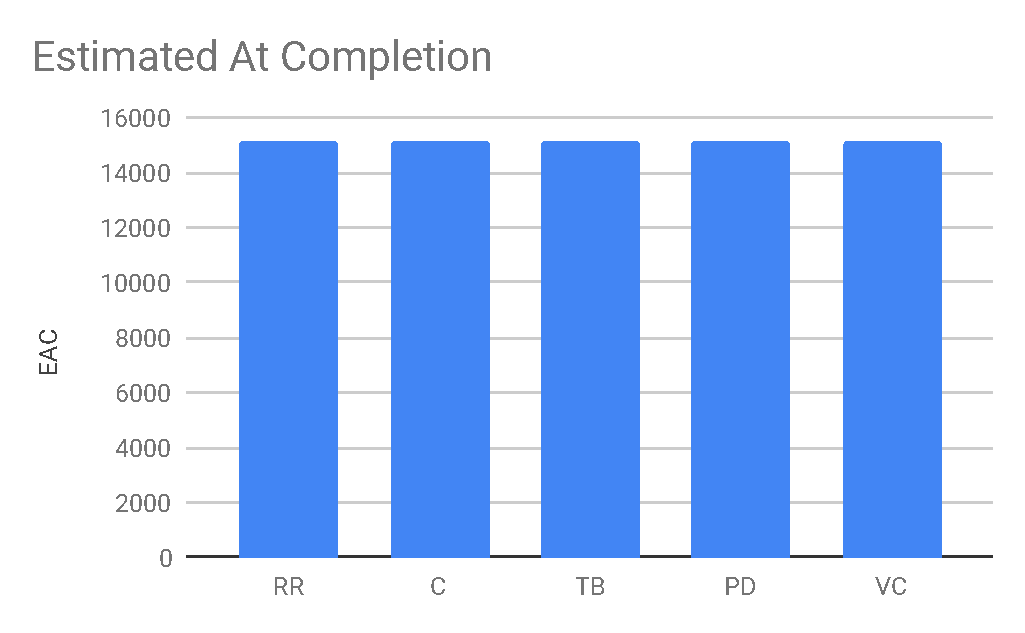
\includegraphics[scale=0.7]{res/images/RA/eac.pdf}
	\caption{Andamento dell'Estimated At Completion durante il progetto}
\end{figure}
\paragraph*{Valutazione}

Le differenze nelle spese sostenute (-144\euro in TB, +355\euro in PB) non sono state tanto gravi da inficiare il preventivo a finire, ragion per cui EAC rimane invariato e di valore pari al preventivo.\\
La soglia prevista del 5\% è pienamente rispettata.

%\subsubsection{Profondità della gerarchia}

\subsubsection{VAC - Variance At Completion}
\begin{figure}[H]
	\centering
	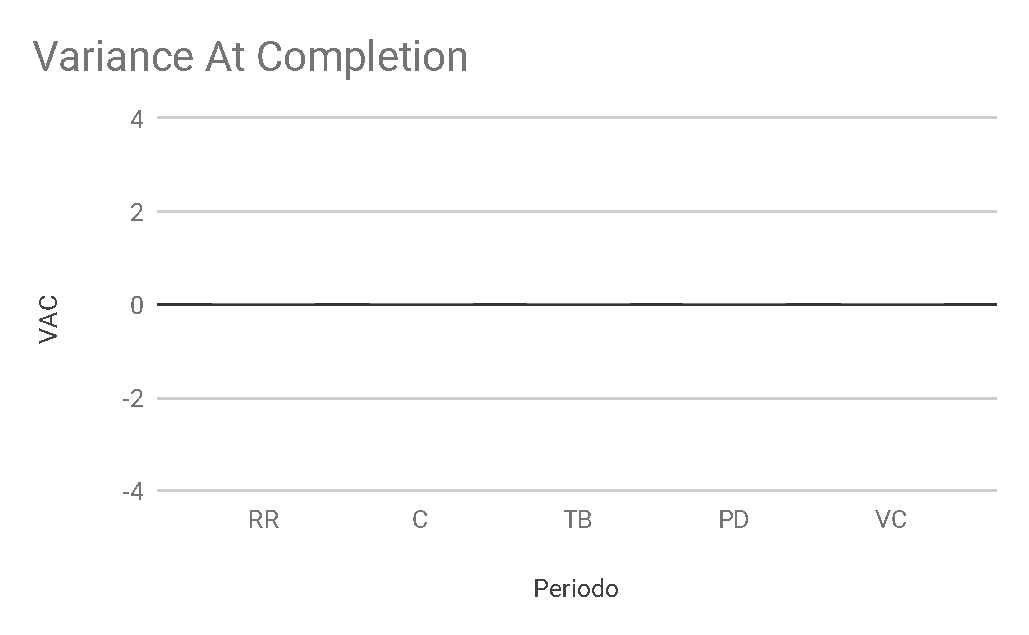
\includegraphics[scale=0.7]{res/images/RA/vac.pdf}
	\caption{Andamento della Variance At Completion durante il progetto}
\end{figure}
\paragraph*{Valutazione}
La differenza tra preventivo e EAC rimane invariata nei periodi e pari a zero; dunque VAC, cioè la percentuale della differenza, è ugualmente invariata e pari a zero. \\
L'obiettivo di avere $VAC \geq 0\%$ è raggiunto.

\subsubsection{EV - Earned Value}
\begin{figure}[H]
	\centering
	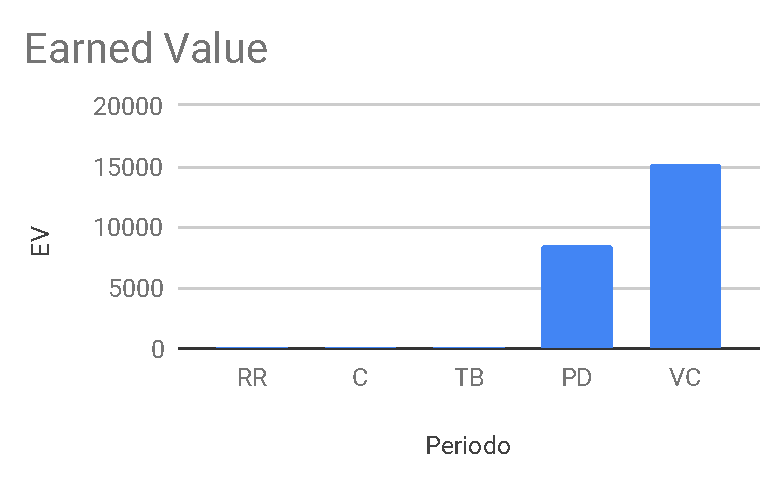
\includegraphics[scale=0.7]{res/images/RA/ev.pdf}
	\caption{Andamento dell'Earned Value durante il progetto}
\end{figure}
\paragraph*{Valutazione}
Possiamo notare che, nonostante il lavoro svolto non ci sia stato alcun guadagno prima della PB. L'EV dipende dalla quantità di obiettivi raggiunti, misurata dal numero di requisiti soddisfatti: ecco spiegata la tardiva produzione di valore.\\
Durante la PB sarebbe stato preferibile aver soddisfatto dimostrabilmente un numero maggiore di requisiti: in mancanza di ciò, in RA avremo un carico di lavoro maggiore rispetto alle attività previste. 

\subsubsection{AC - Actual Cost}
\begin{figure}[H]
	\centering
	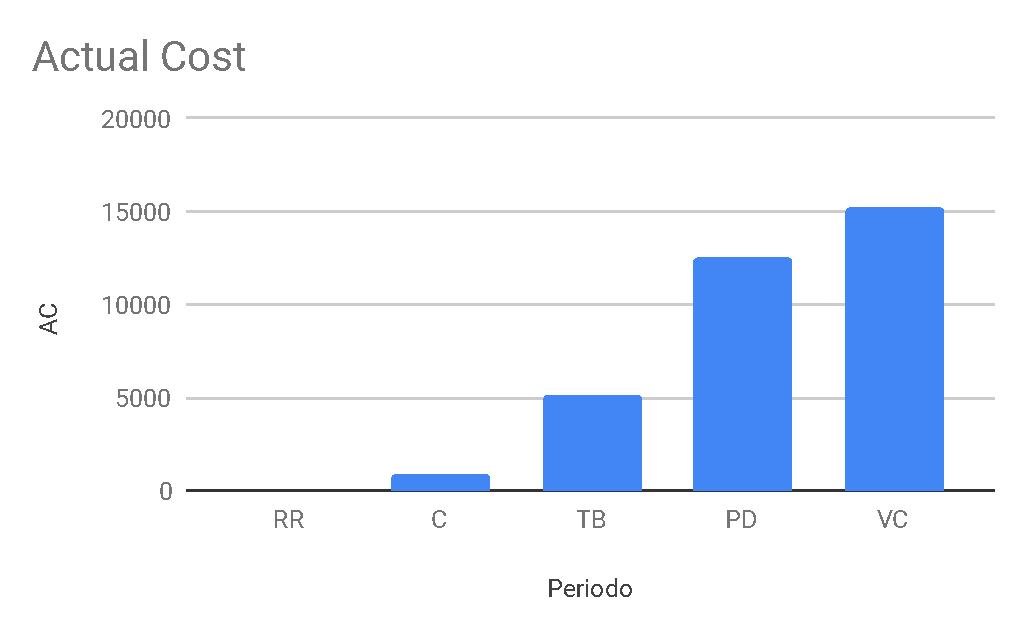
\includegraphics[scale=0.7]{res/images/RA/ac.pdf}
	\caption{Andamento dell'Actual Cost durante il progetto}
\end{figure}
\paragraph*{Valutazione}
Il costo effettivo del lavoro, durante ogni fase, non si è molto discostato da quanto preventivato: dunque la pianificazione svolta risulta adeguata rispetto ai costi del lavoro previsti. \\
Durante la fase di PB, AC ha superato PV, dunque la soglia di ottimalità $0 \leq AC < PV$ è stata infranta. La soglia di accettabilità invece è sempre stata rispettata.

\subsubsection{PV - Planned Value}
% IPOTESI: 20% dei req soddisfatti in TB, 80% in PB, 100% in VC
\begin{figure}[H]
	\centering
	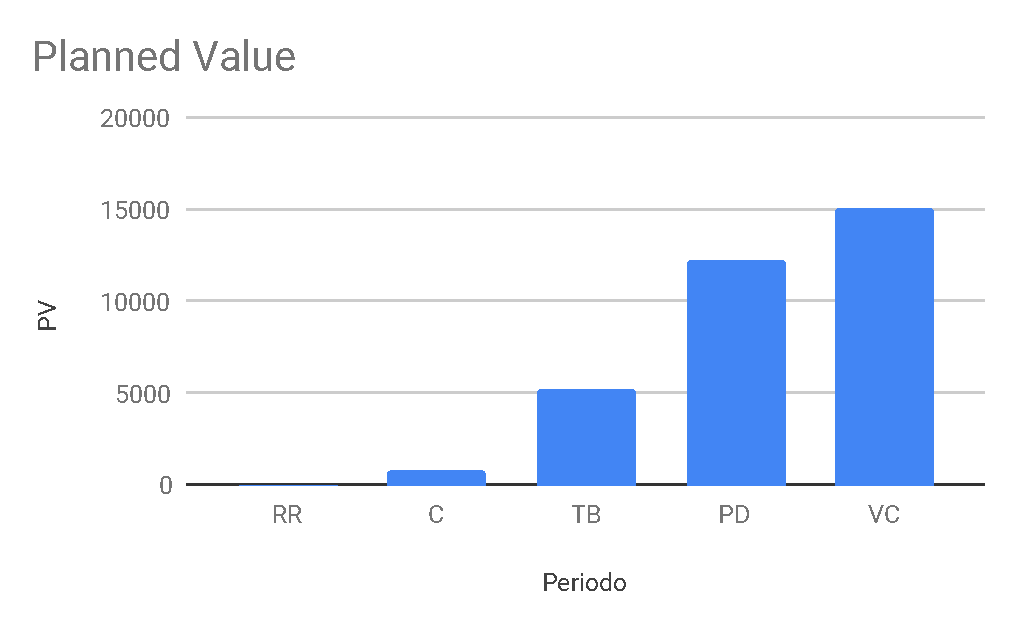
\includegraphics[scale=0.7]{res/images/RA/pv.pdf}
	\caption{Andamento del Planned Value durante il progetto}
\end{figure}
\paragraph*{Valutazione}
Il PV riporta semplicemente il valore del lavoro preventivato fino al momento del calcolo.

\subsubsection{SV - Schedule Variance}
\begin{figure}[H]
	\centering
	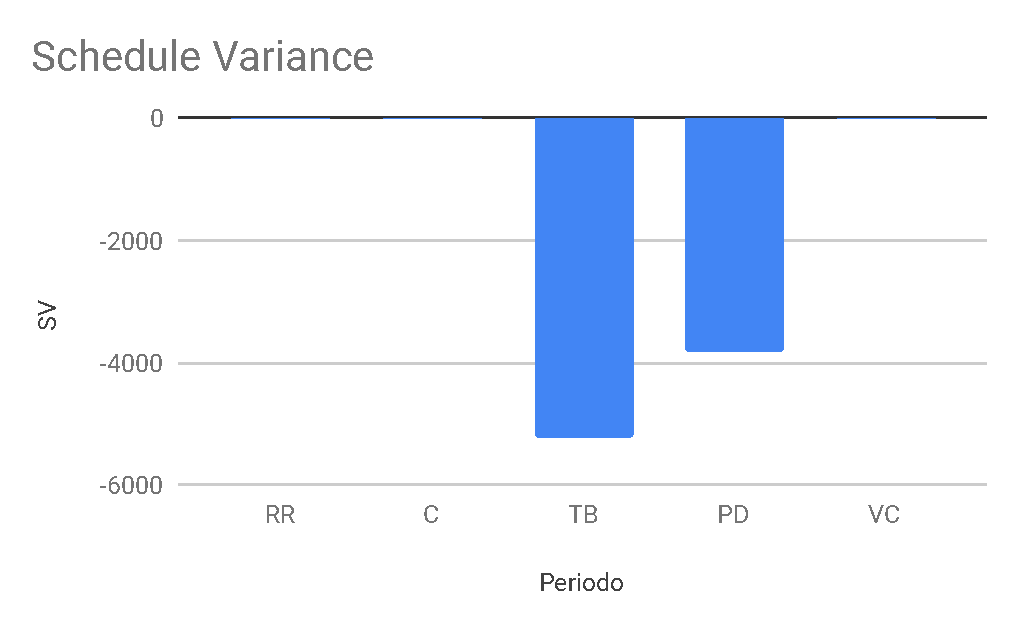
\includegraphics[scale=0.7]{res/images/RA/sv.pdf}
	\caption{Andamento della Schedule Variance durante il progetto}
\end{figure}
\paragraph*{Valutazione}
Durante il periodo di TB il valore è preoccupante: il fatto è che non è stato considerato completato alcun requisito, mentre molte spese erano previste.\\
Durante il periodo di PB sono stati soddisfatti molti requisiti, quindi EV è cresciuto, ma non a sufficienza da coprire le spese previste.\\
Le soglie imposte per la metrica appaiono troppo restrittive, quindi inadeguate rispetto alla pianificazione del progetto.

\subsubsection{CV - Cost Variance}
\begin{figure}[H]
	\centering
	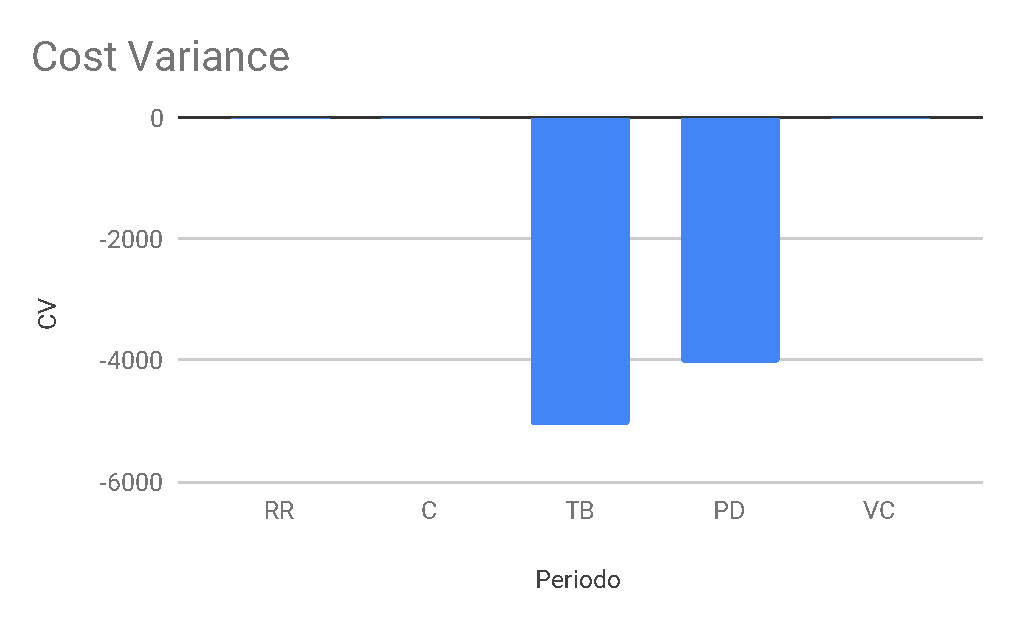
\includegraphics[scale=0.7]{res/images/RA/cv.pdf}
	\caption{Andamento della Cost Variance durante il progetto}
\end{figure}
\paragraph*{Valutazione}
Valgono i ragionamenti fatti in SV per quanto riguarda EV.

%\pagebreak
\subsubsection{Code Coverage}
\paragraph{Statement coverage}\mbox{}\\
\begin{figure}[H]
	\centering
	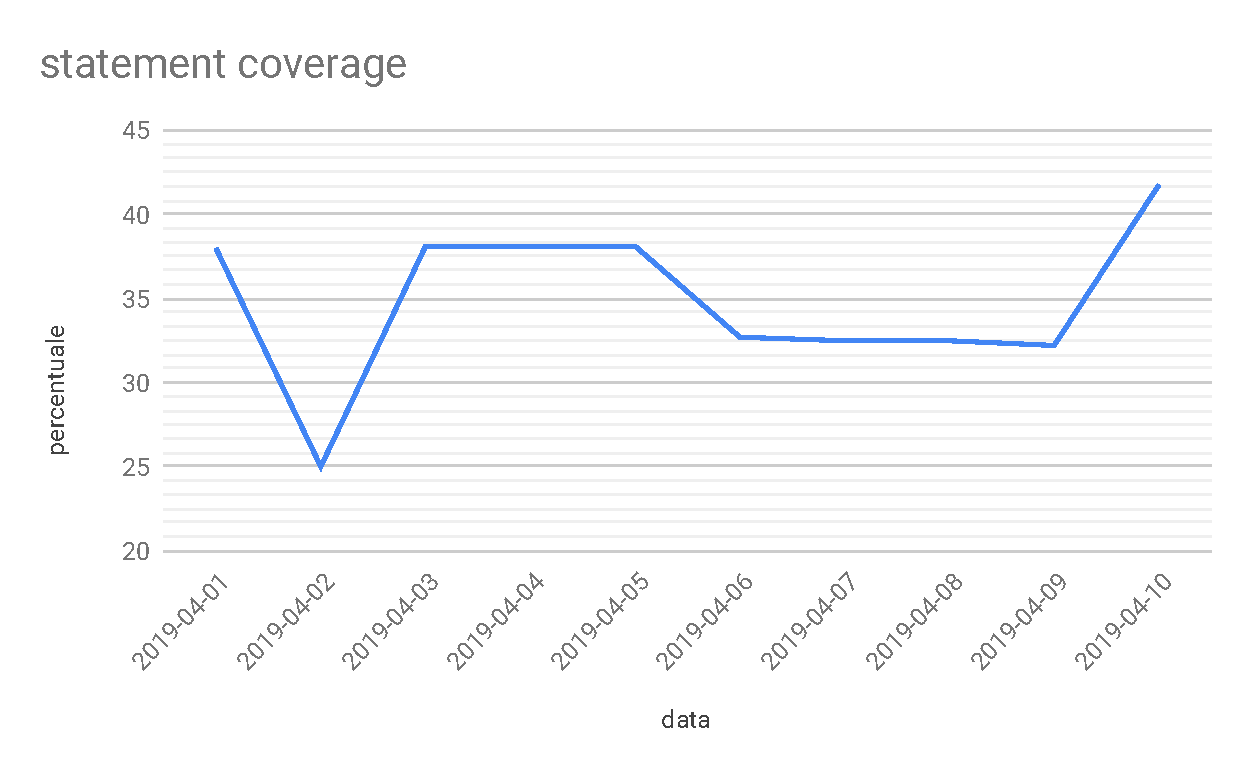
\includegraphics[scale=0.6]{res/images/RA/statement-coverage-RQ.pdf}
	\caption{Statement coverage}
\end{figure}	
\paragraph{Branch coverage}\mbox{}\\
\begin{figure}[H]
	\centering
	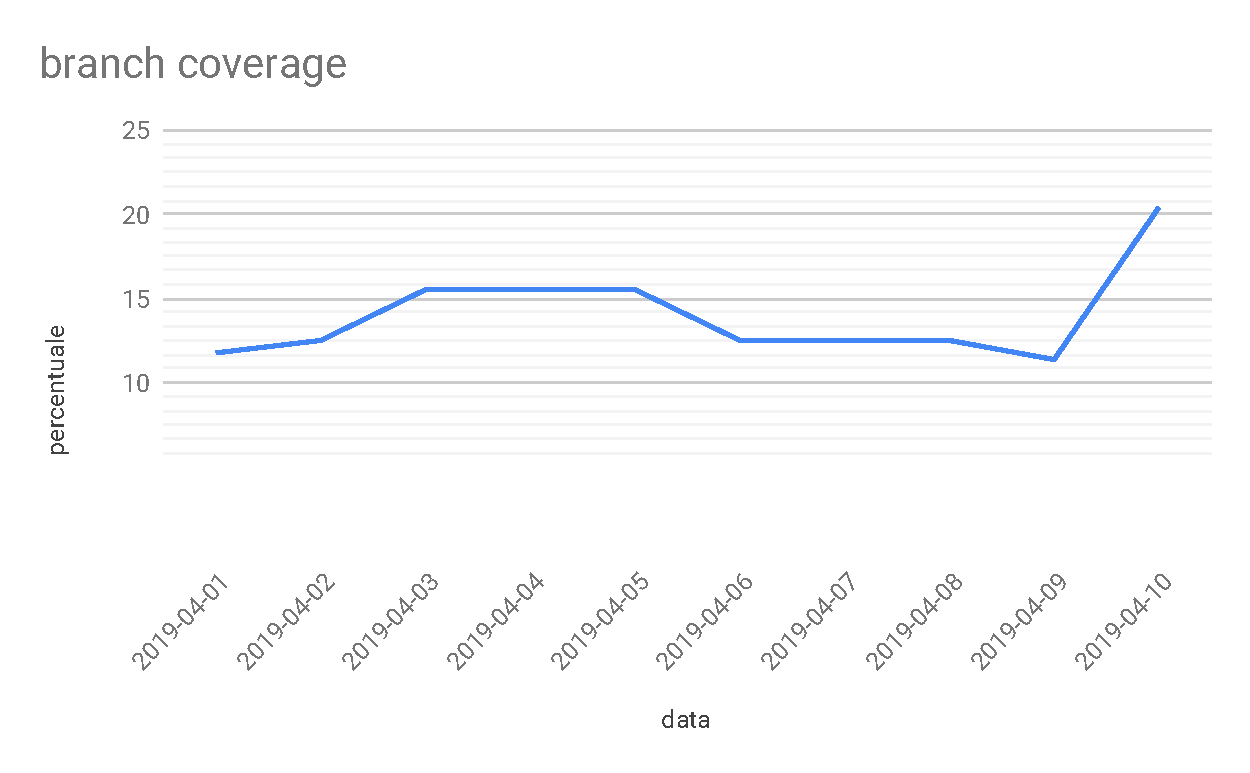
\includegraphics[scale=0.6]{res/images/RA/branch-coverage-RQ.pdf}
	\caption{Branch coverage}
\end{figure}
\paragraph{Function coverage}\mbox{}\\
\begin{figure}[H]
	\centering
	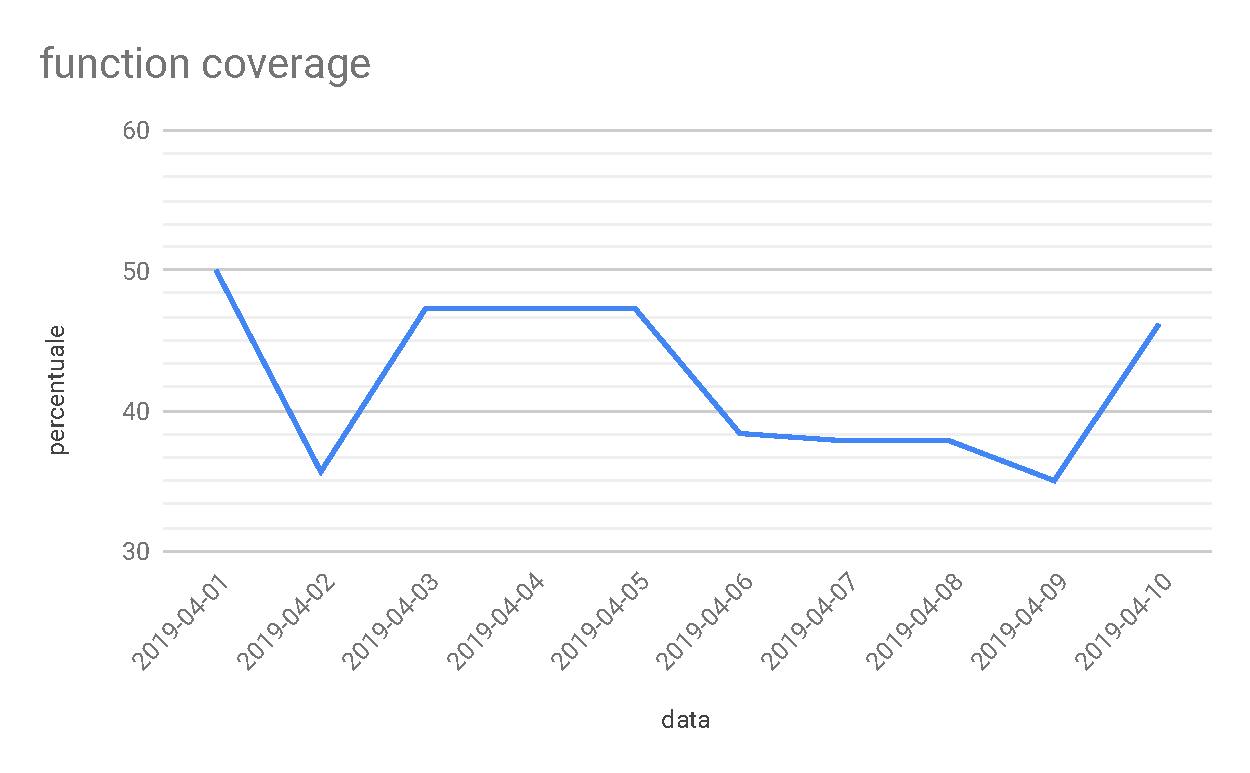
\includegraphics[scale=0.6]{res/images/RA/function-coverage-RQ.pdf}
	\caption{Function coverage}
\end{figure}
\paragraph{Line coverage}\mbox{}\\
\begin{figure}[H]
	\centering
	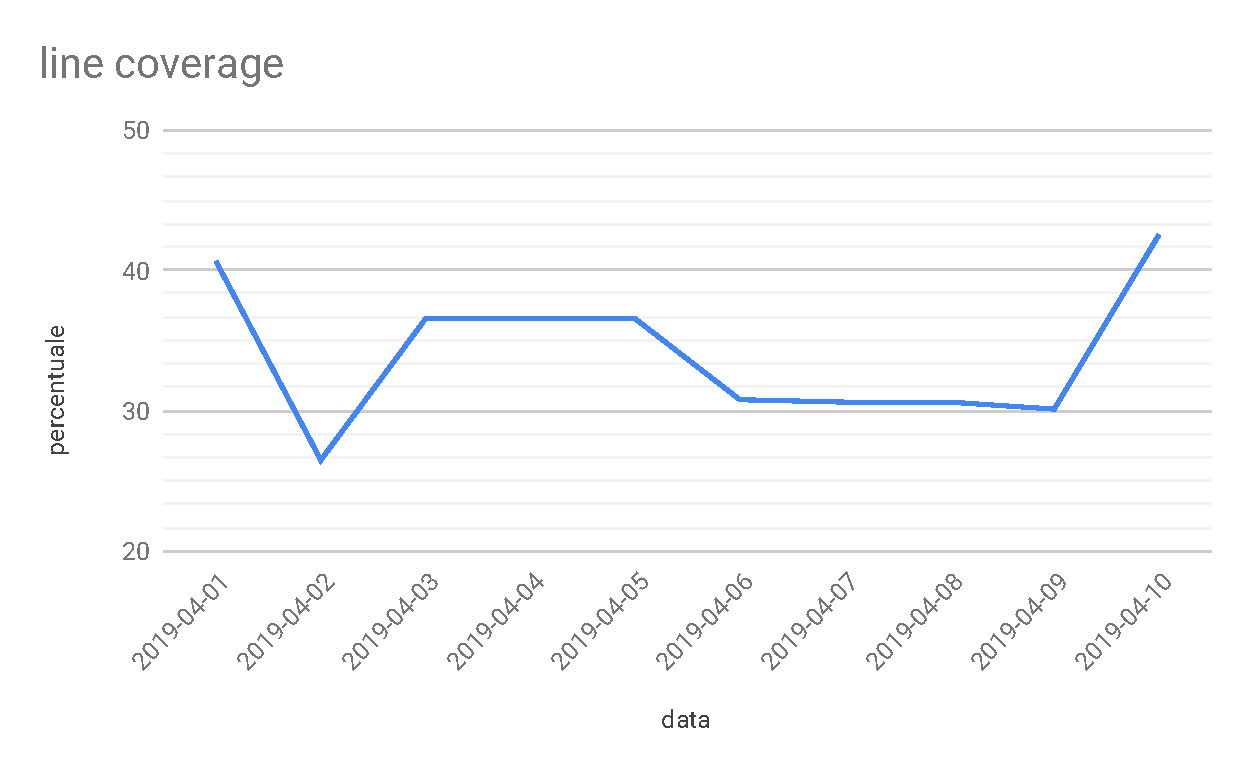
\includegraphics[scale=0.6]{res/images/RA/line-coverage-RQ.pdf}
	\caption{Line coverage}
\end{figure}
\paragraph*{Valutazione complessiva}
Complessivamente la metrica del coverage ha un'andamento prevedibile e si avvicina alle soglie desiderate.
La metrica è stata messa in opera mentre codice e test venivano implementati parallelamente: ecco perché nel periodo iniziale l'andamento del coverage è altalenante.
L'aumento della copertura, a partire dal 10 aprile, corrisponde a una progressione nei test mentre l'ampiezza della codebase rimaneva invariata.
%\subsubsection{Facilità di utilizzo}

\subsubsection{Facilità di comprensione} % == CCR
\begin{figure}[H]
	\centering
	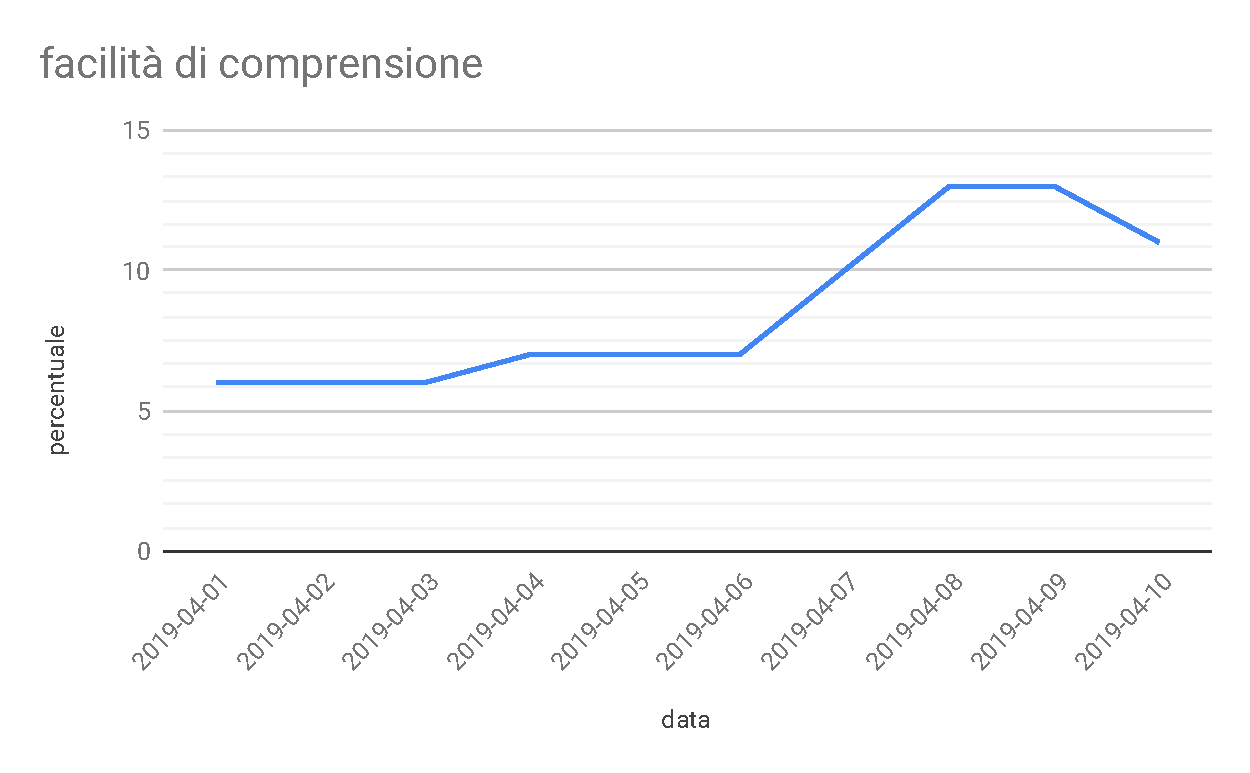
\includegraphics[scale=0.6]{res/images/RA/facilita-di-comprensione.pdf}
	\caption{Facilità di comprensione}
\end{figure}
\paragraph*{Valutazione}
La quantità di commenti rispetto al codice, inizialmente bassa e sregolata, tende alla soglia di accettabilità del 10\% per volere del gruppo di avere un codice chiaro e comprensibile. 

\pagebreak
\subsubsection{Indice di Gulpease}

\begin{longtable}{ >{\centering}p{0.15\textwidth} >{\centering}p{0.10\textwidth}	>{\centering}p{0.1075\textwidth} >{\centering}p{0.10\textwidth} >{\centering}p{0.10\textwidth} >{\centering}p{0.10\textwidth}}
	
	%\hline
	\rowcolor{white}\caption{Indice di Gulpease raggruppato per documento, lungo i periodi da RR a TB}\\
	\rowcolorhead
	\textbf{\color{white}N} 
	& \textbf{\color{white}RR} 
	& \centering\textbf{\color{white}C}
	& \textbf{\color{white}TB}
	& \textbf{\color{white}PD}
	& \textbf{\color{white}VC} 
	\tabularnewline %\hline 	
	
	\textit{Analisi dei requisiti}
	& 67
	& 66
	& 63
	& 63
	& -
	\tabularnewline %\hline 
	
	\textit{Glossario}
	& 71
	& 71
	& 71
	& 71
	& -
	\tabularnewline %\hline 
	
	\textit{Norme di progetto}
	& 65
	& 65
	& 63
	& 66
	& -
	\tabularnewline %\hline 
	
	\textit{Piano di progetto}
	& 68
	& 68
	& 66
	& 67
	& -
	\tabularnewline %\hline 
	
	\textit{Piano di qualifica}
	& 70
	& 70
	& 67
	& 65
	& -
	\tabularnewline %\hline 
	
	\textit{Studio di Fattibilità}
	& 73
	& -
	& -
	& -
	& -
	\tabularnewline %\hline 
	
	\textit{Verbali esterni (media)}
	& 72
	& 72
	& 66
	& 69
	& -
	\tabularnewline %\hline 
	
	\textit{Verbali interni (media)}
	& 74
	& 74
	& 70
	& 73
	& -
\end{longtable}
\begin{figure}[H]
	\centering
	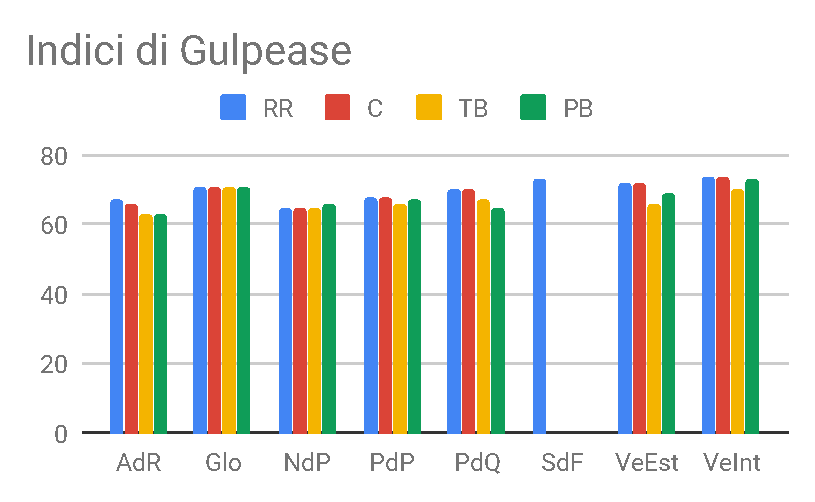
\includegraphics[scale=0.8]{res/images/RA/gulpease.pdf}
	\caption{Indice di Gulpease}
\end{figure}

\paragraph*{Valutazione}
Fino alla fase C l'indice è stato calcolato con uno strumento diverso rispetto alle fasi successive: questo spiega la discordanza tra i valori prima e dopo.
In generale, nonostante l'impegno del gruppo nella semplificazione della sintassi, l'indice non sembra migliorare molto.
Questo può indicare una generale difficoltà nel semplificare documenti di natura tecnica.\\
A una valutazione posteriore, la soglia di ottimalità imposta appare eccessivamente ottimistica: un valore $>80$ infatti indica un testo leggibile con facilità da bambini delle elementari.\\
La soglia di accettabilità invece sono plausibili e rispettate. 

%\subsubsection{Semplicità delle classi}

\subsubsection{SLOC}
\begin{figure}[H]
	\centering
	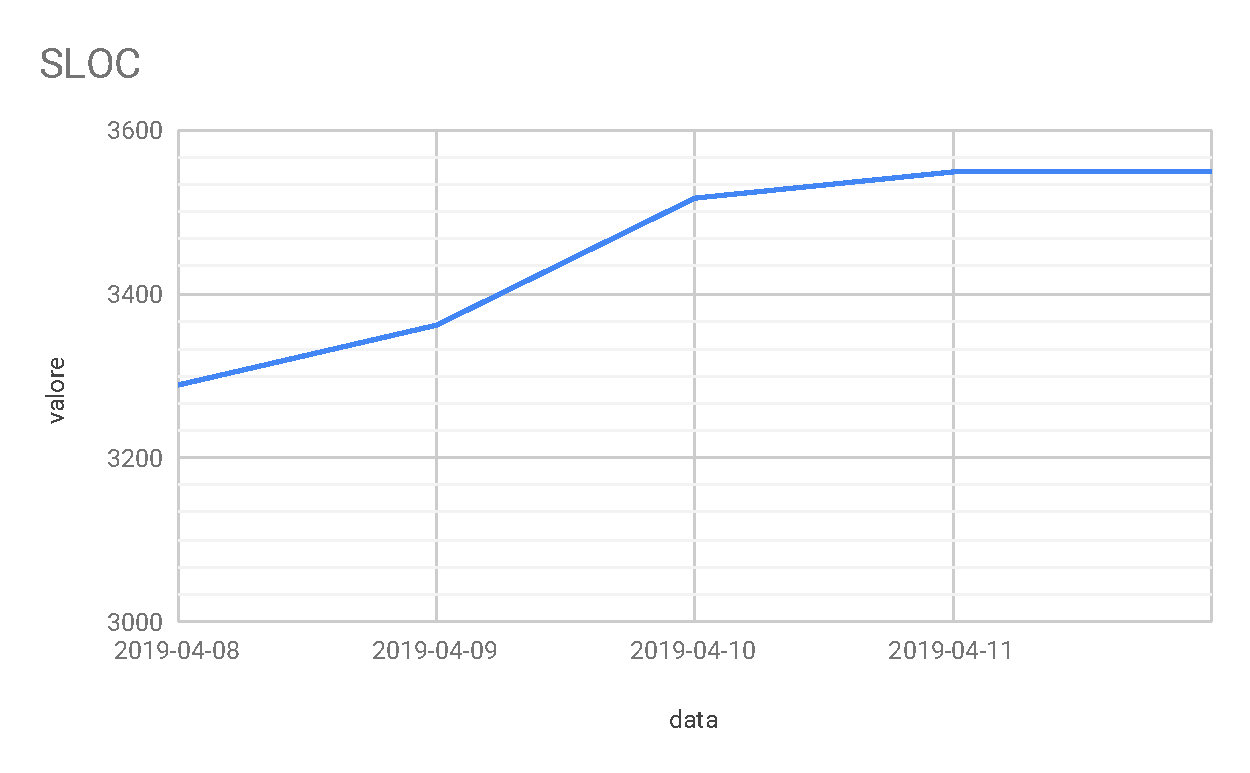
\includegraphics[scale=0.6]{res/images/RA/sloc.pdf}
	\caption{Source lines of code}
\end{figure}
\paragraph*{Valutazione}
Lo SLOC ha un'andamento prevedibile tendente al logaritmo, che indica una stabilità delle righe totali di codice del prodotto man mano che il progetto si avvicina alla fine. Le soglie di accettabilità e ottimalità sono rispettate.


